\documentclass[a4paper, 11pt, titlepage]{article}
\usepackage{graphicx}
\usepackage{pdfpages}
\usepackage{fancybox}
\usepackage[francais]{babel}
\usepackage[utf8]{inputenc}
% \usepackage[T1]{fontenc}
\usepackage{amsmath,amsfonts,amssymb}
\usepackage{fancyhdr}
\usepackage{stackrel}
\usepackage{babel,indentfirst}
\usepackage{xspace}
\usepackage{url}
\usepackage{titling}
\usepackage{listings}
\usepackage{color}
\usepackage{array}
\usepackage{hyperref}
\usepackage{makecell}
\usepackage{tikz}

%\setlength{\parindent}{0pt}
\setlength{\parskip}{1ex}
\setlength{\textwidth}{17cm}
\setlength{\textheight}{24cm}
\setlength{\oddsidemargin}{-.7cm}
\setlength{\evensidemargin}{-.7cm}
\setlength{\topmargin}{-.5in}


\lstset{
  sensitive=f,
  morestring=[d]",
  showstringspaces=false,
  basicstyle=\small\ttfamily,
  keywordstyle=\bf\small,
  commentstyle=\itshape,
  stringstyle=\sf,
  extendedchars=true,
  columns=[c]fixed
}



\predate{
\begin{center}
}
\postdate{
\\
\vspace{1.5cm}
\includegraphics[scale=0.7]{imag.png}
\end{center}}


\title {{ {\huge Compte rendu du projet ACVL / Web }} }

\author{\Large Equipe 14 \\
\\
    {\sc Aboubacar}~Salim\\
    {\sc Demets}~Jules-Eugène\\
    {\sc Gouttefarde}~Léo\\
    {\sc Rey}~Simon
}

\date{Jeudi 14 Avril 2016}

\lhead{Projet ACVL / Web}
\rhead{Compte rendu}

\begin{document}
\pagestyle{fancy}
\maketitle

\tableofcontents
\newpage

% \begin{center}
% \section* {Introduction }
% \end{center}


% (a) Document d’analyse :
% — acteurs, diagramme de cas d’utilisations et description de ces cas d’utilisations, illustrées par des diagrammes de séquence système pertinents.
% — diagramme de classes d’analyse.

\section {Analyse}


Le sujet présente une application pour une association de jeux de rôle. 

\subsection{Acteurs}

Seuls deux types d'acteur peuvent intervenir dans cette application : les joueurs eux mêmes (c'est-à-dire les rôlistes) ainsi que les meneurs de jeu, qui dirigent les parties.

\subsection{Cas d'utilisation}

\subsubsection{Description des différents cas d'utilisation}

Voici les différents cas d'utilisation de l'application issus du cahier des charges, ils sont résumés dans un diagramme à la fin de cette section.

\begin{enumerate}
    \item Un joueur peut consulter la biographie d'un personnage 
        \begin{enumerate}
            \item  S'il possède le personnage il peut voir les paragraphes privés de la biographie.
            \item De même le meneur de jeu d'un personnage peut voir les paragraphes privés du dit personnage.
        \end{enumerate}
    \item Un joueur peut révéler des paragraphes secrets des biographies des personnage qu'il possède 
    \begin{enumerate}
        \item  L'application doit demander une validation pour cette action.            
    \end{enumerate}
        \includegraphics[scale=0.5]{sequence/RevelerParagAnalyse.png}
      \item Un joueur peut créer un personnage 
      \begin{enumerate}
        \item  Le joueur doit alors indiquer : nom, date de naissance, profession ainsi qu'une biographie initiale
        \item Le joueur peut soumettre le personnage ainsi créé à un meneur de jeu
        \item Le meneur de jeu peut accepter le personnage, il peut lire la biographie (y compris les parties secrètes).
      \end{enumerate}
      \item Le meneur de jeu, ou un joueur, peut ajouter des épisodes à la biographie d'un de ses personnages 
      \begin{enumerate}
        \item Il en spécifie la date
        \item Il peut spécifier une aventure à laquelle est rattaché cet épisode. 
        \item  Il peut sauvegarder l'épisode en cours de rédaction.
        \item Il peut reprendre l'édition.
        \item Il peut supprimer l'épisode en cours d'édition
        \item Il peut le valider
        \item Une fois validé par le joueur et le meneur de jeu l'épisode devient définitif : il ne peut plus être modifier.
      \end{enumerate}
      \textit{De ce fait il est impossible de valider un épisode si le personnage n'a pas de meneur de jeu associé.}
      \begin{center}\includegraphics[scale=0.5]{sequence/AjouterEpisodeBiographie.png} \end{center}
    \item Un joueur peut proposer d'organiser une partie
    \begin{enumerate}
        \item  Il indique alors : titre, univers dans lequel se déroule la partie, situation initiale date et lieu
        \item La proposition est alors visible par tous.
        \item Le meneur de jeu peut ajouter ou enlever des personnages, ceux-ci doivent être du même univers que la partie et il doit être le meneur de jeu des personnages
        \item La proposition peut être supprimée
    \end{enumerate}
    \item Le meneur de jeu peut saisir un résumé des événements et indiquer la fin de la partie
    \begin{enumerate}
        \item Les éléments relatifs à la partie ne sont dés lors plus modifiables.
        \item La partie devient une aventure pouvant apparaitre dans la biographie des personnages.
    \end{enumerate}
    \item Un joueur peut céder son personnage
    \begin{enumerate}
        \item Il indique le joueur bénéficiaire
    \end{enumerate}
    \item Un joueur peut changer le meneur de jeu d'un de ses personnages
    \begin{enumerate}
        \item Le nouveau meneur de jeu doit accepter.
        \item Ce transfert ne peut avoir lieu que si le personnage n'est pas impliqué dans une partie en cours.
    \end{enumerate}
    \includegraphics[scale=0.5]{sequence/ChangerleMJ.png}
    \end{enumerate}

\subsubsection{Diagramme des cas d'utilisation}

\begin{center}
    \includegraphics[scale=0.7,angle=90]{analyse/usecases}
\end{center}

\subsection{Diagramme de classes d'analyse}
Le sujet fournit une description des différents "objets" de l'application : partie, aventure, personnage, univers, biographie, épisode, paragraphe ... 
Voici le diagramme de classe d'analyse que nous en avons tiré.\\
\textit{Nous avons considéré qu'une partie était simplement une aventure en cours (nous aurions pu faire de l'héritage mais l'avantage semblait mince par rapport aux inconvénients de la conversion d'une partie en aventure ). \\
    De même nous n'avons pas distingués les classes joueur et meneur de jeu : un joueur est meneur de jeu s'il est engagé dans les relations qui caractérisent un meneur de jeu (parties menés, personnages dont il est le meneur ...) Cela se justifie par le caractère dynamique de ce  statut : un joueur peut facilement devenir meneur de jeu ou arrêter de l'être, être un meneur de jeu semblait donc être plutôt une propriété dynamique des joueurs. }
\begin{center}\includegraphics[scale=0.7]{analyse/classes.pdf} \end{center}







% (b) Document de conception :
% — L’architecture générale modèle-vue-contrôleur est imposée, mais indiquez comment vous la
% mettez en œuvre : quels sont les contrôleurs et les vues, comment tout s’articule-t-il.
% — Conception détaillée : diagramme de classes logicielles, diagrammes de séquence, diagrammes
% d’états-transitions si cela est pertinent. Ces diagrammes doivent être cohérents entre eux et
% avec l’implémentation. Il est inutile de fournir des diagrammes illisibles ou qui n’apportent
% aucune information ; il peut être en revanche utile d’ajouter un minimum de texte explicatif
% le cas échéant.

\section {Conception}

\subsection {Architecture}

\subsubsection {Contrôleurs, Servlets}

Nous avons segmenté la gestion de l'application en différents Servlets contrôleurs :
\begin{itemize}
\item
\lstinline!AventureCtrl! : Servlet de gestion des différentes aventures

\item
\lstinline!BiographieCtrl! : Servlet de gestion des différentes biographies

\item
\lstinline!EpisodeCtrl! : Servlet de gestion des différents épisodes

\item
\lstinline!Main! : Contrôleur principal de l'application

\item
\lstinline!ParagrapheCtrl! : Servlet de gestion des différents paragraphes

\item
\lstinline!PersonnageCtrl! : Servlet de gestion des différents personnages
\end{itemize}


\subsubsection {Vue}

Les vues sont organisées en dossiers correspondant aux différents contrôleurs. Nous avons également tiré parti de l'héritage de vues JSP à l'aide de fichiers tag JSP (squelette principal contenu dans le fichier \lstinline!src/main/webapp/WEB-INF/tags/wrapper.tag!), et utilisé la librairie JSTL au sein des différentes vues.


\subsubsection {Modèle}

Nous avons modélisé chaque table relationnelle par une classe Java correspondante pour facilement gérer l'encapsulation en objets des différents éléments.


\subsubsection {DAO}

Pour les accès à la base de données, nous avons utilisé des DAO correspondant aux différentes classes du modèle ainsi que des classes abstraites correspondantes pour aider à la spécification originelle des différentes méthodes et faciliter la collaboration.



\subsection {Détail de la conception}

\subsection {Diagramme de classes UML}

\includegraphics[scale=0.7]{conception/classes}

\subsection {Diagramme d'état transition pour la création d'épisodes, de personnages, ou de parties}

\includegraphics[scale=0.6]{conception/creation-episodes-perso-parties.jpg}

\subsection {Diagramme de classes logicielles}

% TODO



\section {Détails techniques}

L'application est normalement protégée contre tout type de faille XSS (via JSTL) et également des attaques par injection SQL.

De plus la vérification des droits d'accès pour chaque type d'action a bien été implémentée, ainsi que la gestion des différentes erreurs dont le message reste intégré au design de l'application.

La gestion unicode des caractère a également été correctement gérée dans l'ensemble de l'application.

Pour finir, les requêtes ont été écrites de manière à pouvoir assurer les accès concurrents (sérialisation des requêtes qui modifient la base de données), à l'aide de transactions (pas d'autocommit) et avec annulation des transactions en cas d'erreur.




\section {Manuel d'utilisation}

\subsection {Mise en route}

Différents joueurs sont installés dans la base d'origine.
Pour commencer, il suffit de se connecter avec les identifiants ci-dessous.

\subsubsection {Meneur admin}

Login : \lstinline!admin!, mot de passe : \lstinline!admin17Lord!


\subsubsection {Meneur Clara}

Login : \lstinline!Clara!, mot de passe : \lstinline!Vasto42!


\subsubsection {Joueur James}

Login : \lstinline!James!, mot de passe : \lstinline!james007tb!


\subsubsection {Meneur Max}

Login : \lstinline!Max!, mot de passe : \lstinline!max71Lord!




\subsection {Utilisation}

L'application est composée d'une barre horizontale de navigation munie de différents sous-menus : Personnages, Parties et MJ.

Chacun d'entre-eux permet d'accéder à plusieurs liens correspondant, permettant l'accès aux différentes fonctionnalités de l'application.


\subsubsection {Menu Personnages}

Ce menu permet d'accéder aux fonctionnalités suivantes :

\begin{itemize}
\item
Créer un personnage : Permet de créer un personnage

\item
Liste des personnages : Affiche la liste des personnages de l'application

\item
Mes personnages : Affiche la liste des personnages possédés

\end{itemize}


\subsubsection {Menu Parties}

Ce menu permet d'accéder aux fonctionnalités suivantes :

\begin{itemize}
\item
Proposer une partie : Permet de créer une nouvelle partie

\item
Liste des parties : Affiche la liste des parties de l'application

\item
Mes parties : Affiche la liste des parties auxquelles a participé l'utilisateur, ainsi que le personnage utilisé

\end{itemize}


\subsubsection {Menu MJ}

\begin{itemize}
\item
Parties menées : Affiche la liste des parties menées

\item
Personnages menés : Affiche la liste des personnages menées

\item
Personnages à valider : Affiche la liste des personnages à valider

\item
Transferts à valider : Affiche la liste des personnages à transférer

\item
Episodes à valider : Affiche la liste des épisodes à valider

\end{itemize}




\subsubsection {Gestion d'un personnage}

En cliquant sur l'un des personnages d'une liste, on arrive à sa page personnalle. Celle-ci permet de visualiser les différentes informations du personnage, de modifier sa profession, et contient des liens vers sa biographie et les parties auxquelles il a participé.

De plus, il possible de faire valider / transférer le personnage s'il est invalide ou ne participe pas à une partie en cours, de même il possible de céder le personnage via une liste déroulante (sauf s'il participe à une partie en cours, car sinon des joueurs pourraient se retrouver avec plusieurs personnages dans une seule partie en cours).

C'est notamment sur cette même page que les meneurs de jeu peuvent accepter une demande de transfert ou de validation.


\subsubsection {Gestion de la biographie}

La biographie est éditable si l'on est meneur ou propriétaire du personnage concerné.

Il suffit alors de cliquer sur les boutons "Nouvel épisode", "Nouveau paragraphe", et autres pour compléter, modifier ou valider des parties de la biographie.

Un bouton révéler permet notamment de rendre les paragraphes secrets publics, avec une demande de confirmation dynamique et une implémentation {\sc ajax} de la fonctionnalité révéler.


\subsubsection {Gestion d'une partie}

En cliquant sur les parties d'une liste, on arrive à leur page personnalisée. Celle-ci permet de visualiser les différentes informations de la partie (ou aventure si elle s'est terminée), et aussi d'accéder à la liste des participants (avec des boutons pour retirer des personnages si l'on en est le meneur).

Le meneur peut également ajouter des participants à l'aide d'une liste déroulante, terminer la partie en inscrivant un résumé des événements dans la fenêtre dynamique qui apparaît, ou encore la supprimer si elle n'est pas encore finie (avec demande de confirmation dynamique).


% Parler des titres dynamiques (composition avec le titre de chaque page)
% et de la déconnexion




% (d) Bilan sur les outils de modélisation utilisés, en particulier les problèmes rencontrés, ainsi que
% les solutions trouvées. Il vous est demandé dans cette partie de bien préciser les logiciels, en particulier les modeleurs UML que vous avez utilisés.

\section {Bilan sur les outils de modélisation utilisés}

Au cours de ce projet nous avons utilisé différents outils de modélisation.

Au niveau des modeleurs UML, il n'est pas évident de trouver des outils gratuits de bonne qualité, et nous avons finalement choisi d'utiliser l'outil GenMyModel qui permet une modélisation simple et collaborative. Un autre outil de relativement bonne qualité aurait pu être PlantUML, mais il a le désavantage de ne pas être entièrement graphique. Nous avons également testé ArgoUML, mais ce logiciel n'était pas de très bonne qualité.

Certains diagrammes ont également été réalisés à l'aide de Visual Studio (diagramme des cas d'utilisation), ou encore de Web Sequence Diagrams (diagrammes de séquence).




\end{document}


